\chapter{HASIL DAN PEMBAHASAN}
\label{chap:hasildanpembahasan}

% Ubah bagian-bagian berikut dengan isi dari pengujian dan analisis


Pada penelitian ini dipaparkan hasil pengujian berupa implementasi Unreal Engine 5 yang dapat menjalankan sistem dari \emph{Smart Contract Sharing Data}, serta melakukan pengujian terkait
dengan data audio yang diload selama proses sistem berjalan hingga ke tahap pemutaran audio.

\section{Skenario Pengujian}
Pengujian dilakukan dengan melakukan langkah-langkah yang telah ditulis pada bab sebelumnya. Pengujian dimulai dengan melakukan testing method-method yang ada di smart contract.
Fungsi-fungsi yang akan dicoba adalah fungsi yang dibuat sendiri untuk mempermudah proses integrasi. Pengujian dilakukan dengan melibatkan 2 buah akun yang sudah dibuat sebelumnya
menggunakan metamask. Kemudian untuk method-method tersebut juga akan diuji performa dari penggunaan gas dan ETH-nya. Lalu akan dilakukan pengujian integrasi dari Unreal Engine 5.
Pengujian integrasi meliputi berhasil tidaknya melakukan pemutaran audio yang sudah di-\emph{mint} sebelumnya.

\subsection{Hasil Pembuatan Wallet Account}
Pembuatan wallet account dilakukan dengan Metamask. Pada platform metamask dapat dilakukan pembuatan akun dengan menginstall extension browsernya. Setelah terbuat akunnya maka perlu
digunakan faucet untuk mengisi ETH. ETH yang didapat adalah sejumlah 13 GoerliETH. ETH ini sudah lebih dari cukup untuk digunakan. Kemudian dibuat juga akun kedua dan diisikan dengan GoerliETH.
Akun kedua juga dapat digunakan untuk pengujian.


\subsection{Hasil dan Pengujian Method Smart Contract}
Smart Contract yang dibuat dapat digunakan untuk mint NFT. Deployment dilakukan dengan Environment Injected Provider Metamask.
Metamask yang digunakan adalah akun yang sudah dibuat sebelumnya. Contract yang dibuat dideploy sudah digunakan untuk mint NFT.
Untuk pengujian method \texttt{mint}, dilakukan dulu proses deploy dengan menggunakan remix IDE. Contract dideploy di Ganache untuk melakukan pengujian secara lokal karena apabila dilakukan deployment di
Metamask maka ETH yang digunakan akan sulit untuk didapatkan kembali. Berikut ini adalah tabel dari hasil pengujian method \texttt{mint}.
\begin{longtable}{|c|c|}
  \caption{Hasil Pengujian Method \texttt{mint}}
  \label{tb:UjiMint}                              \\
  \hline
  \rowcolor[HTML]{C0C0C0}
  \textbf{URI}              & \textbf{Keterangan} \\
  \hline
  HTTP URL yang berisi JSON & Sukses              \\
  HTTP URL random           & Sukses              \\
  String random             & Sukses              \\
  String kosong             & Gagal               \\
  \hline
\end{longtable}

Pada bagian string kosong akan gagal karena diberikan guard sehingga jika tidak diberikan input maka akan terjadi error.
Sementara untuk string random seperti string yang bukan HTTP URL tidak gagal karena tidak diberikan guard ataupun kondisional yang melakukan
pengecekan terhadap data yang diberikan.

Kemudian untuk bagian method \texttt{getAllTokens} maka akan dilakukan pengujian apakah jumlah id yang dikembalikan sesuai dengan jumlah URI yang sudah di \texttt{mint}.

Kegunaan dari method \texttt{getAllTokens} adalah untuk melakukan query jumlah uri yang ada di blockchain. Maka akan dilakukan pemanggilan \texttt{mint} terlebih dahulu
sebelum melakukan pengujian \texttt{getAllTokens}.

\begin{longtable}{|c|c|}
  \caption{Hasil Pengujian Method \texttt{getAllTokens}}
  \label{tb:UjiGetAllTokens}                                                              \\
  \hline
  \rowcolor[HTML]{C0C0C0}
  \textbf{Jumlah Pemanggilan Mint} & \textbf{Panjang Nilai Balikan \texttt{getAllTokens}} \\
  \hline
  1                                & 1                                                    \\
  2                                & 2                                                    \\
  3                                & 3                                                    \\
  4                                & 4                                                    \\
  5                                & 5                                                    \\
  6                                & 6                                                    \\
  7                                & 7                                                    \\
  8                                & 8                                                    \\
  \hline
\end{longtable}

Dari hasil pengujian dapat dilihat hasilnya adalah sesuai ekspektasi.
Ketika method mint dipanggil sejumlah 1 kali, maka panjang nilai yang dikembalikan oleh method \texttt{getAllTokens} adalah
1. Ketika method mint dipanggil sejumlah 2 kali, maka panjang nilai yang dikembalikan oleh method \texttt{getAllTokens} adalah
2. Ketika method mint dipanggil sejumlah 3 kali, maka panjang nilai yang dikembalikan oleh method \texttt{getAllTokens} adalah
3. Ketika method mint dipanggil sejumlah 4 kali, maka panjang nilai yang dikembalikan oleh method \texttt{getAllTokens} adalah
4. Ketika method mint dipanggil sejumlah 5 kali, maka panjang nilai yang dikembalikan oleh method \texttt{getAllTokens} adalah
5. Ketika method mint dipanggil sejumlah 6 kali, maka panjang nilai yang dikembalikan oleh method \texttt{getAllTokens} adalah
6. Ketika method mint dipanggil sejumlah 7 kali, maka panjang nilai yang dikembalikan oleh method \texttt{getAllTokens} adalah
7. Ketika method mint dipanggil sejumlah 8 kali, maka panjang nilai yang dikembalikan oleh method \texttt{getAllTokens} adalah
8.

Kemudian untuk pengujian method selanjutnya adalah pengujian method \texttt{getAllTokensURI}.
Untuk method ini akan mengembalikan balikan array yang berisi
URI yang sudah disimpan dengan method \texttt{mint} yang sudah pernah dipanggil sebelumnya. Hasil yang diharapkan adalah dengan memanggil method ini maka URI-URI yang sudah pernah
di mint sebelumnya akan dikembalikan dalam bentuk array.

\begin{longtable}{|p{2.5in}|p{2.5in}|}
  \caption{Hasil Pengujian Method \texttt{getAllTokensURI}}
  \label{tb:UjiGetAllTokensURI}                                                                                                                                                                                                                                 \\
  \hline
  \rowcolor[HTML]{C0C0C0}
  \textbf{Mint URI}                                                                                                            & \textbf{Balikan}                                                                                                               \\
  \hline
  https://bafybeu.ipfs.w3s.link/nft-1.json                                                                                     & [https://bafybeu.ipfs.w3s.link/nft-1.json]                                                                                     \\
  https://bafybeu.ipfs.w3s.link/nft-2.json                                                                                     & [https://bafybeu.ipfs.w3s.link/nft-2.json]                                                                                     \\
  https://bafybeu.ipfs.w3s.link/nft-1.json, https://bafybeu.ipfs.w3s.link/nft-2.json                                           & [https://bafybeu.ipfs.w3s.link/nft-1.json, https://bafybeu.ipfs.w3s.link/nft-2.json]                                           \\
  Tidak pernah memanggil method Mint                                                                                           & []                                                                                                                             \\
  https://bafybeu.ipfs.w3s.link/nft-1.json, https://bafybeu.ipfs.w3s.link/nft-2.json, https://bafybeu.ipfs.w3s.link/nft-3.json & [https://bafybeu.ipfs.w3s.link/nft-1.json, https://bafybeu.ipfs.w3s.link/nft-2.json, https://bafybeu.ipfs.w3s.link/nft-3.json] \\
  \hline
\end{longtable}

Dari pemanggilan method-method getAllTokensURI hasilnya adalah sesuai dengan yang diharapkan. Apabila dilakukan mint sebanyak 2 kali maka akan dikembalikan juga sebanyak 2 dan berisikan uri-uri yang sudah pernah di mint sebelumnya.
Apabila dilakukan mint sebanyak 3 kali maka akan dikembalikan juga sebanyak 3 dan berisikan uri-uri yang sudah pernah di mint sebelumnya.
Apabila dilakukan mint sebanyak 4 kali maka akan dikembalikan juga sebanyak 4 dan berisikan uri-uri yang sudah pernah di mint sebelumnya.
Apabila dilakukan mint sebanyak 5 kali maka akan dikembalikan juga sebanyak 5 dan berisikan uri-uri yang sudah pernah di mint sebelumnya.
Method ini akan berguna untuk melakukan pemanggilan di Unreal Engine 5.
Apabila fungsi ini dipanggil oleh Unreal Engine 5 blueprint maka akan dibaca berupa array URI.

Kemudian untuk pengujian method tokenURI akan dilakukan dengan memanggil method mint dan kemudian menggunakan indexnya untuk memanggil  method tokenURI ini. Method ini akan
menggunakan parameter tokenId yang mana adalah urutan dilakukannya mint. Index ini bersifat incremental yang artinya URI pertama memiliki index 0, URI kedua memiliki index 1,
URI ketiga memiliki index 3, URI keempat memiliki index 4, dan URI kelima memiliki index 5, dan seterusnya.

Berikut adalah tabel hasil pengujian method \texttt{tokenURI}

\begin{longtable}{|p{0.5in}|p{2.2in}|p{0.5in}|p{2.2in}|}
  \caption{Hasil Pengujian Method \texttt{tokenURI}}
  \label{tb:UjiTokenURI}                                                                                                                      \\
  \hline
  \rowcolor[HTML]{C0C0C0}
  \textbf{Mint-ke} & \textbf{URI}                             & \textbf{Parameter method tokenURI} & \textbf{Balikan method tokenURI}         \\
  \hline
  1                & https://bafybeu.ipfs.w3s.link/nft-1.json & 1                                  & https://bafybeu.ipfs.w3s.link/nft-1.json \\
  2                & https://bafybeu.ipfs.w3s.link/nft-1.json & 2                                  & https://bafybeu.ipfs.w3s.link/nft-1.json \\
  3                & https://bafybeu.ipfs.w3s.link/nft-1.json & 3                                  & https://bafybeu.ipfs.w3s.link/nft-1.json \\
  4                & https://bafybeu.ipfs.w3s.link/nft-1.json & 4                                  & https://bafybeu.ipfs.w3s.link/nft-1.json \\
  5                & https://bafybeu.ipfs.w3s.link/nft-1.json & 5                                  & https://bafybeu.ipfs.w3s.link/nft-1.json \\
  6                & https://bafybeu.ipfs.w3s.link/nft-1.json & 6                                  & https://bafybeu.ipfs.w3s.link/nft-1.json \\
  7                & https://bafybeu.ipfs.w3s.link/nft-1.json & 7                                  & https://bafybeu.ipfs.w3s.link/nft-1.json \\
  8                & https://bafybeu.ipfs.w3s.link/nft-1.json & 8                                  & https://bafybeu.ipfs.w3s.link/nft-1.json \\
  9                & https://bafybeu.ipfs.w3s.link/nft-1.json & 9                                  & https://bafybeu.ipfs.w3s.link/nft-1.json \\
  10               & https://bafybeu.ipfs.w3s.link/nft-1.json & 10                                 & https://bafybeu.ipfs.w3s.link/nft-1.json \\
  11               & https://bafybeu.ipfs.w3s.link/nft-1.json & 11                                 & https://bafybeu.ipfs.w3s.link/nft-1.json \\
  12               & https://bafybeu.ipfs.w3s.link/nft-1.json & 12                                 & https://bafybeu.ipfs.w3s.link/nft-1.json \\
  13               & https://bafybeu.ipfs.w3s.link/nft-1.json & 13                                 & https://bafybeu.ipfs.w3s.link/nft-1.json \\
  14               & https://bafybeu.ipfs.w3s.link/nft-1.json & 14                                 & https://bafybeu.ipfs.w3s.link/nft-1.json \\
  15               & https://bafybeu.ipfs.w3s.link/nft-1.json & 15                                 & https://bafybeu.ipfs.w3s.link/nft-1.json \\
  0                & https://bafybeu.ipfs.w3s.link/nft-1.json & 100                                & <ERROR> Invalid token ID                 \\
  \hline
\end{longtable}

Pada kondisi normal pemanggilan method tokenURI sesuai dengan yang dikehendaki. Pemanggilan tokenURI akan mengembalikan uri dengan index yang diberikan.
Namun jika token ID yang diberikan tidak ditemukan di blockchain, maka akan terjadi error Invalid token ID.
Hal ini merupakan \emph{behavior} yang dikehendaki karena memang jika tidak ditemukan URI seharusnya dihasilkan error.
Jika tidak   diberikan  error maka bisa terjadi \emph{undefined behavior} pada saat digunakan di Unreal Engine 5.

Pada pengujian selanjutnya adalah pengujian gas pada setiap method-method diatas. Pengujian ini bertujuan untuk mengukur
efisiensi smart contract yang digunakan pada penelitian ini.

\subsection{Hasil Pengujian Estimasi Gas}

Pengujian ini menyajikan hasil total keseluhan biaya gas yang diperlukan dalam melakukan proses transaksi pengiriman nominal Ether dari pengirim ke penerima.
Pengujian ini dilakukan dengan cara memanggil masing-masing method yang akan diujikan lalu mencatat nilai konsumsi gasnya.
Dengan menggunakan \emph{Ganache} dan juga dilakukan pada network \emph{Goerli} dan juga \emph{Sepolia} yang menerapkan konsensus Proof of Work.

\begin{figure}[H]
  \centering

  % Ubah dengan nama file gambar dan ukuran yang akan digunakan
  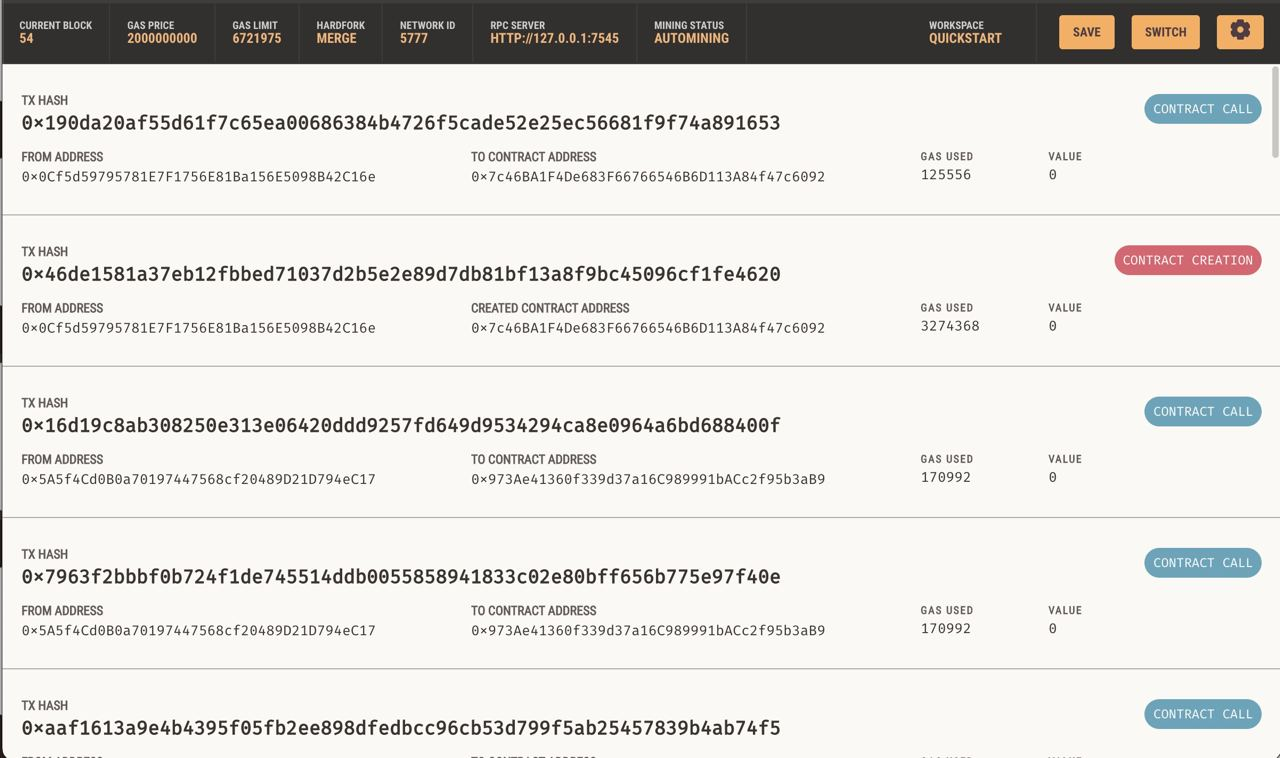
\includegraphics[scale=0.35]{gambar/ganache-uji-gas.jpg}

  % Ubah dengan keterangan gambar yang diinginkan
  \caption{Transaksi blockchain di Ganache}
  \label{fig:ganachegastest}
\end{figure}

Tujuan dari pengujian ini adalah untuk mengetahui berapa besar biaya gas yang dibutuhkan untuk menjalankan proses sistem pada Smart Contract yang sudah dibuat.
Proses dari pengujian ini sama seperti dengan Ganache network, hanya saja setiap proses sistem yang berjalan, lamanya waktu terkonfirmasi pada Metamask ditemukan variasi, yang mana
sangat berbeda dengan Ganache yang tidak memiliki jeda. Untuk method-method yang bersifat read only atau tidak payable dan tidak melakukan write operation tidak dilakukan
uji gas karena method-method tersebut tidak menggunakan gas untuk dieksekusi.

\begin{enumerate}
  \item
        \textbf{Deployment Gas}

        Pengujian estimasi gas dimulai dari jaringan Ganache. Tabel dibawah ini menunjukan estimasi gas yang dibutuhkan untuk melakukan proses deploy Smart Contract pada Ganache

        \begin{longtable}{|c|c|c|}
          \caption{Hasil Pengujian Deploy Smart Contract}
          \label{tb:UjiDeploy}                                                                             \\
          \hline
          \rowcolor[HTML]{C0C0C0}
          \textbf{\emph{Blockchain Network}} & \textbf{\emph{Gas Used}} & \textbf{\emph{Gas Price (Gwei)}} \\
          \hline
          Ganache                            & 3274368                  & 2.772126468                      \\
          Goerli                             & 3275354                  & 2.500000024                      \\
          Sepolia                            & 3275354                  & 2.500000012                      \\
          \hline
        \end{longtable}

        \begin{longtable}{|c|c|c|}
          \caption{Hasil Pengujian Deploy Smart Contract di \emph{Ganache}}
          \label{tb:UjiDeployGanache}                                                                \\
          \hline
          \rowcolor[HTML]{C0C0C0}
          \textbf{\emph{Percobaan ke}} & \textbf{\emph{Gas Used}} & \textbf{\emph{Gas Price (Gwei)}} \\
          \hline
          1                            & 3274368                  & 2.769504978                      \\
          2                            & 3274368                  & 2.77037599                       \\
          3                            & 3274368                  & 2.760107065                      \\
          4                            & 3274368                  & 2.760947704                      \\
          5                            & 3274368                  & 2.761791060                      \\
          6                            & 3274368                  & 2.762637142                      \\
          7                            & 3274368                  & 2.763485958                      \\
          8                            & 3274368                  & 2.764337517                      \\
          9                            & 3274368                  & 2.758433902                      \\
          10                           & 3274368                  & 2.759269134                      \\
          11                           & 3274368                  & 2.760107034                      \\
          12                           & 3274368                  & 2.77037569                       \\
          13                           & 3274368                  & 2.760108232                      \\
          14                           & 3274368                  & 2.761792302                      \\
          15                           & 3274368                  & 2.762633213                      \\
          \hline
        \end{longtable}

        Dari hasil tabel yang didapatkan diatas, didapati bahwa penggunaan gas cukup besar karena proses melakukan deploy memang membutuhkan resource yang tidak sedikit.
        Gas Used pada jaringan lokal Ganache juga lebih besar daripada di jaringan Goerli dan Sepolia. Pada tabel \ref{tb:UjiDeployGanache} juga dilakukan 10 kali percobaan
        yang mana hasilnya dapat disimpulkan bahwa gas price di jaringan lokal ganache lebih besar daripada Goerli dan Sepolia pada saat pengujian proses deployment smart contract.

  \item
        \textbf{Minting Gas}

        Pengujian efisiensi gas selanjutnya adalah pengujian saat melakukan minting token atau proses pembuatan NFT untuk menyimpan data URI.
        Proses ini sendiri memanggil method \texttt{mint} dan karena method ini bersifat write dan payable maka penggunaan gas nya pun akan lebih
        banyak dibandingkan method yang bersifat write. Pengujian ini akan dilakukan dengan jaringan lokal ganache dan juga jaringan Goerli dan Sepolia.
        Berikut ini adalah table hasil pengujian efisiensi gas untuk pemanggilan method mint pada smart contract.

        \begin{longtable}{|c|c|c|}
          \caption{Hasil Pengujian Gas Mint Smart Contract}
          \label{tb:UjiGasMint}                                                                            \\
          \hline
          \rowcolor[HTML]{C0C0C0}
          \textbf{\emph{Blockchain Network}} & \textbf{\emph{Gas Used}} & \textbf{\emph{Gas Price (Gwei)}} \\
          \hline
          Ganache                            & 170992                   & 2.526306790                      \\
          Goerli                             & 125580                   & 2.500000016                      \\
          Sepolia                            & 125568                   & 2.500000016                      \\
          \hline
        \end{longtable}

        \begin{longtable}{|c|c|c|}
          \caption{Hasil Pengujian Gas Mint di \emph{Ganache}}
          \label{tb:UjiGasMintGanache}                                                               \\
          \hline
          \rowcolor[HTML]{C0C0C0}
          \textbf{\emph{Percobaan ke}} & \textbf{\emph{Gas Used}} & \textbf{\emph{Gas Price (Gwei)}} \\
          \hline
          1                            & 170992                   & 2.526306790                      \\
          2                            & 170992                   & 2.529847969                      \\
          3                            & 170992                   & 2.533865829                      \\
          4                            & 170992                   & 2.538424537                      \\
          5                            & 170992                   & 2.543596897                      \\
          6                            & 170992                   & 2.549465512                      \\
          7                            & 170992                   & 2.556124107                      \\
          8                            & 170992                   & 2.764337517                      \\
          9                            & 170992                   & 2.758433902                      \\
          10                           & 170992                   & 2.759269134                      \\
          11                           & 170992                   & 2.526303233                      \\
          12                           & 170992                   & 2.529832132                      \\
          13                           & 170992                   & 2.533847239                      \\
          14                           & 170992                   & 2.538491925                      \\
          15                           & 170992                   & 2.543581052                      \\
          \hline
        \end{longtable}

        Dari tabel \ref{tb:UjiGasMintGanache} diatas dapat diketahui bahwasanya Gas Used pada method mint cukup besar untuk standard
        blockchain smart contract. Kemudian untuk pemakaian gas yang dilakukan di jaringan lokal ganache lebih besar daripada di jaringan Goerli
        maupun Sepolia. Hal ini memperkuat hasil dari uji deployment yang dilakukan sebelumnya karena disana juga pemakaian gas yang ada di jaringan lokal
        Ganache. Gas Price ditentukan oleh tingkat penggunaan jaringan blockchain tersebut, sehingga semakin banyak pengguna yang mengakses jaringan dari suatu
        blockchain maka akan semakin banyak juga gas price yang akan dikonsumsi.
\end{enumerate}


\subsection{Hasil Pembuatan Metadata dengan IPFS}
Pengujian untuk IPFS dilakukan dengan cara melakukan pencocokan metadata dengan OpenSea. Metadata yang distandarkan oleh OpenSea akan digunakan dalam sistem.

Metadata yang dibuat di IPFS sudah dapat diakses melalui gatewaynya. Contohnya untuk nft-1.json adalah sebagai berikut.

\begin{figure}[H]
  \centering

  % Ubah dengan nama file gambar dan ukuran yang akan digunakan
  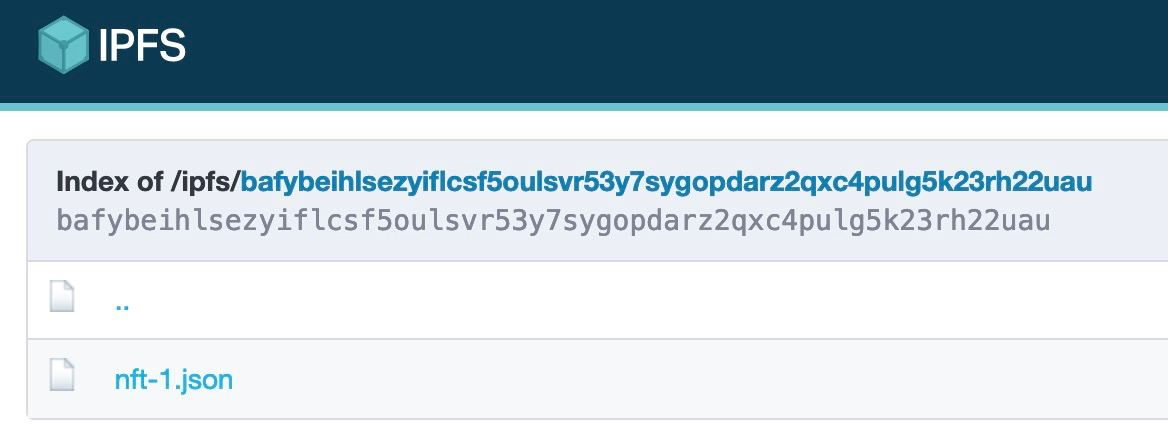
\includegraphics[scale=0.4]{gambar/nftjsonuploaded.jpg}

  % Ubah dengan keterangan gambar yang diinginkan
  \caption{Tampilan IPFS nft-1.json yang sudah diupload}
  \label{fig:ipfsjsonuploaded}
\end{figure}

Hasil dari pembacaan metadata pada OpenSea dengan jaringan testnet adalah dapat terbaca. Jika tidak digunakan standar metadata yang sudah menjadi konvensi
maka tidak akan terbaca oleh OpenSea apa yang sudah dituliskan pada metadata JSON yang diberikan pada jaringan blockchain OpenSea dalam bentuk mint file. Kemudian untuk
URI nya sendiri haruslah berupa URI valid, apabila tidak valid maka OpenSea juga tidak dapat membaca URI yang menyebabkan tidak dapat membaca metadata tersebut karena file metadata yang berupa JSON tersebut tersimpan
di dalam URI yang diberikan.

\begin{figure}[H]
  \centering

  % Ubah dengan nama file gambar dan ukuran yang akan digunakan
  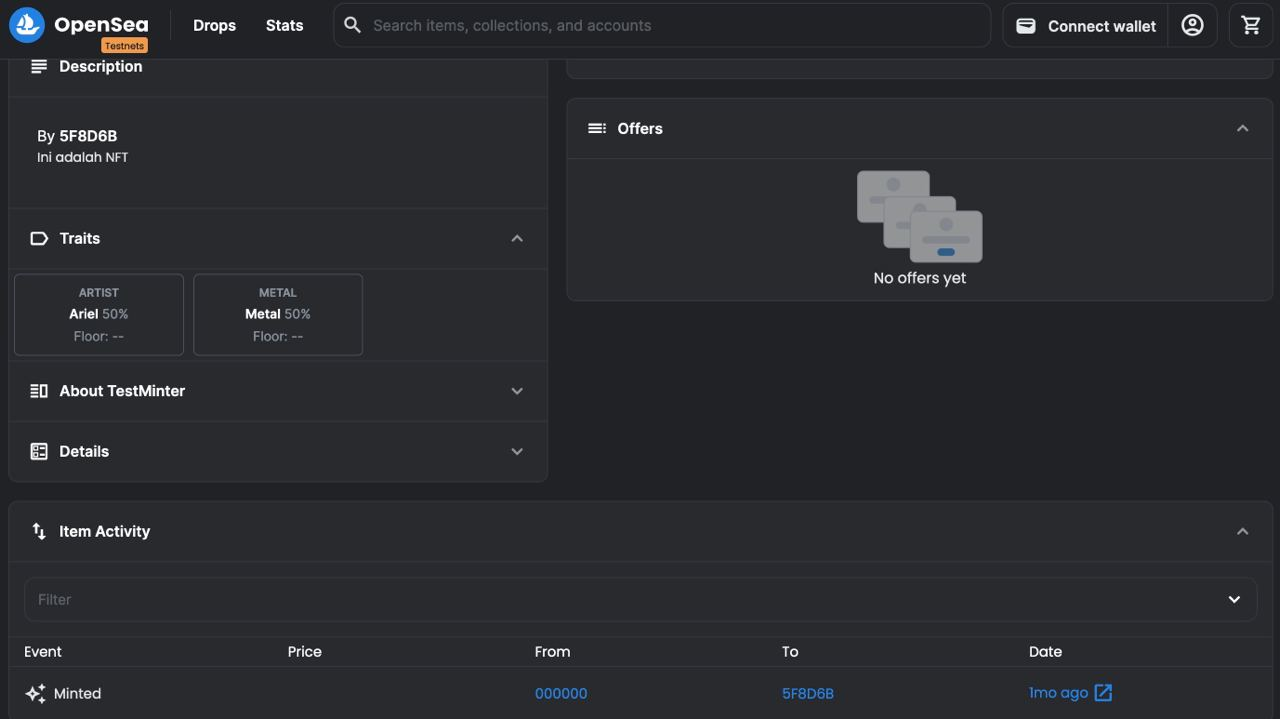
\includegraphics[scale=0.4]{gambar/opensea-uji.jpg}

  % Ubah dengan keterangan gambar yang diinginkan
  \caption{Tampilan OpenSea yang berhasil membaca metadata}
  \label{fig:openseatest}
\end{figure}

Penelitian ini menggunakan metadata yang sudah distandarkan oleh OpenSea, namun tidak ada pengecekan untuk formatnya itu sendiri sehingga apabila dimasukkan format yang salah maka integrasi dengan Unreal Engine 5 akan
gagal dan menyebabkan error yang detailnya akan dijelaskan pada pengujian-pengujian berikutnya.

\subsection{Hasil Mint NFT}
Pengujian ini berbeda dengan pengujian method \texttt{mint} yang ada pada pengujian-pengujian sebelumnya. Pada pengujian ini proses mint yang dimaksud adalah
proses dimana dilakukan deployment smart contract ke jaringan blockchain Goerli. Nantinya jaringan ini akan digunakan untuk integrasi dengan Unreal Engine 5.

Deployment smart contract ke jaringan Goerli dilakukan dengan akun yang sudah berisikan cukup GoerliETH karena proses deployment juga membutuhkan Ether.

\begin{longtable}{|c|c|}
  \caption{Hasil Pengujian Deploy ke Goerli berdasarkan Ether}
  \label{tb:UjiGoerliETH}                         \\
  \hline
  \rowcolor[HTML]{C0C0C0}
  \textbf{Jumlah GoerliETH} & \textbf{Keterangan} \\
  \hline
  12.5                      & Sukses              \\
  0                         & Gagal               \\
  0.001                     & Gagal               \\
  \hline
\end{longtable}

Dari tabel \ref{tb:UjiGoerliETH} dapat disimpulkan bahwa diperlukan jumlah GoerliETH yang memadai untuk dilakukannya proses deployment smart contract.
Minimum GoerliETH  untuk dilakukan deployment adalah 0.01 untuk batas amannya. Namun perlu diperhatikan juga bahwa proses mint URI tetap membutuhkan GoerliETH juga
sehingga perlu disiapkan GoerliETH yang cukup. GoerliETH didapat secara mining pada faucet-faucet yang tersedia di internet.

Hasil dari mint nft sudah dapat digunakan untuk integrasi Unreal Engine 5. ABI dapat dilihat pada compiler Remix IDE.
\begin{figure}[H]
  \centering

  % Ubah dengan nama file gambar dan ukuran yang akan digunakan
  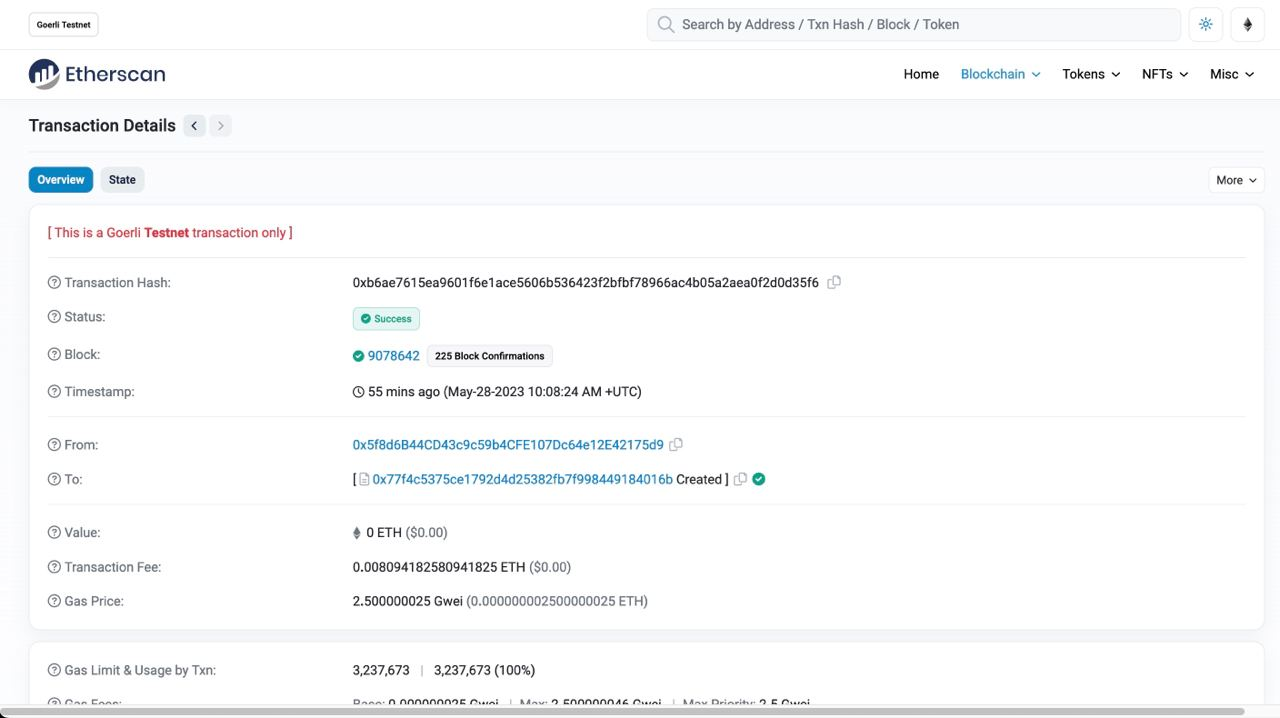
\includegraphics[scale=0.35]{gambar/etherscan-deploy.jpg}

  % Ubah dengan keterangan gambar yang diinginkan
  \caption{Etherscan dari hasil transaction mint NFT}
  \label{fig:etherscandeploy}
\end{figure}

\subsection{Hasil Pembuatan Project Pada Unreal Engine 5}
Project unreal engine 5 yang sudah dibuat dapat memberikan environment visual yang dapat melakukan visualisasi audio maupun game.

\begin{figure}[H]
  \centering

  % Ubah dengan nama file gambar dan ukuran yang akan digunakan
  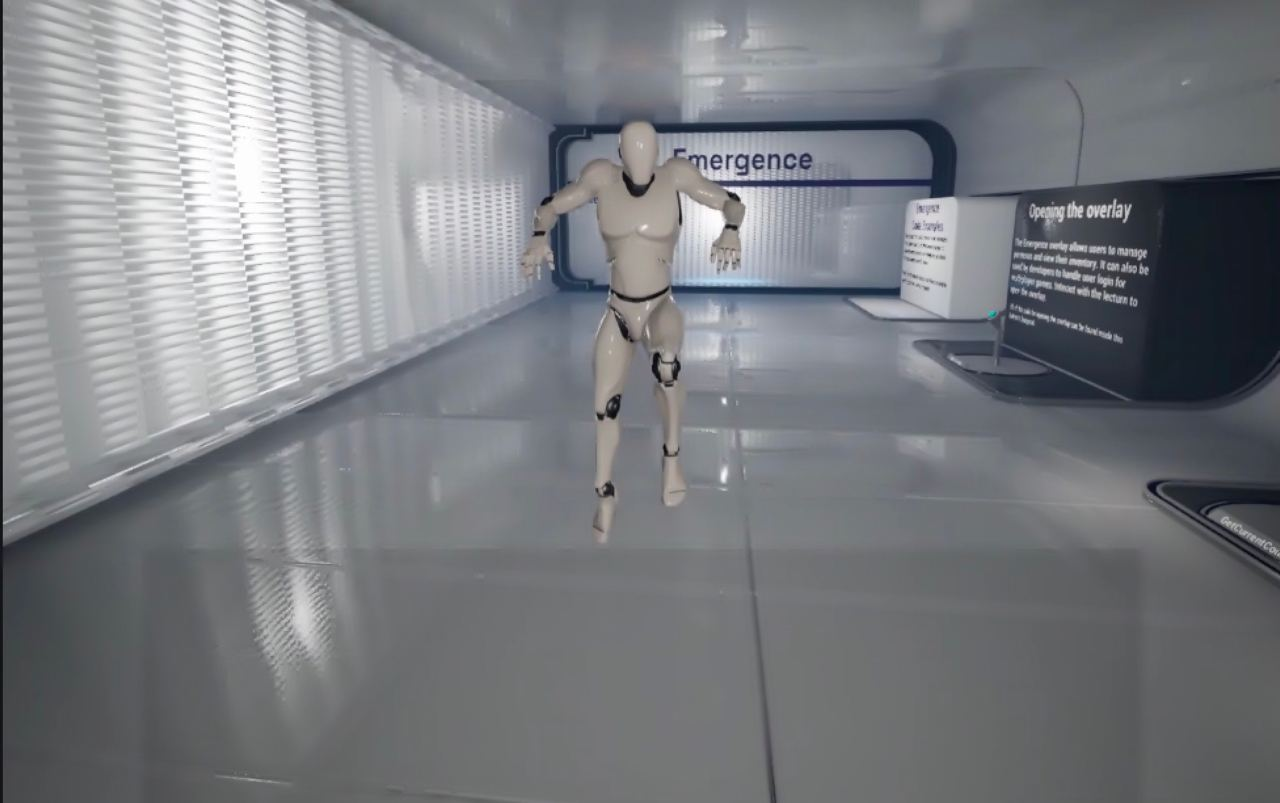
\includegraphics[scale=0.35]{gambar/ue5project.jpg}

  % Ubah dengan keterangan gambar yang diinginkan
  \caption{Tampilan project unreal engine 5}
  \label{fig:ue5project}
\end{figure}

\subsection{Hasil Integrasi Kontrak dengan Unreal Engine 5}

Setelah diintegrasikan dengan blueprint maka di lingkungan virtual unreal engine 5 sudah dapat memutar audio yang didapatkan dari NFT.
Blueprint yang digunakan adalah sebagai berikut.

\begin{figure}[H]
  \centering

  % Ubah dengan nama file gambar dan ukuran yang akan digunakan
  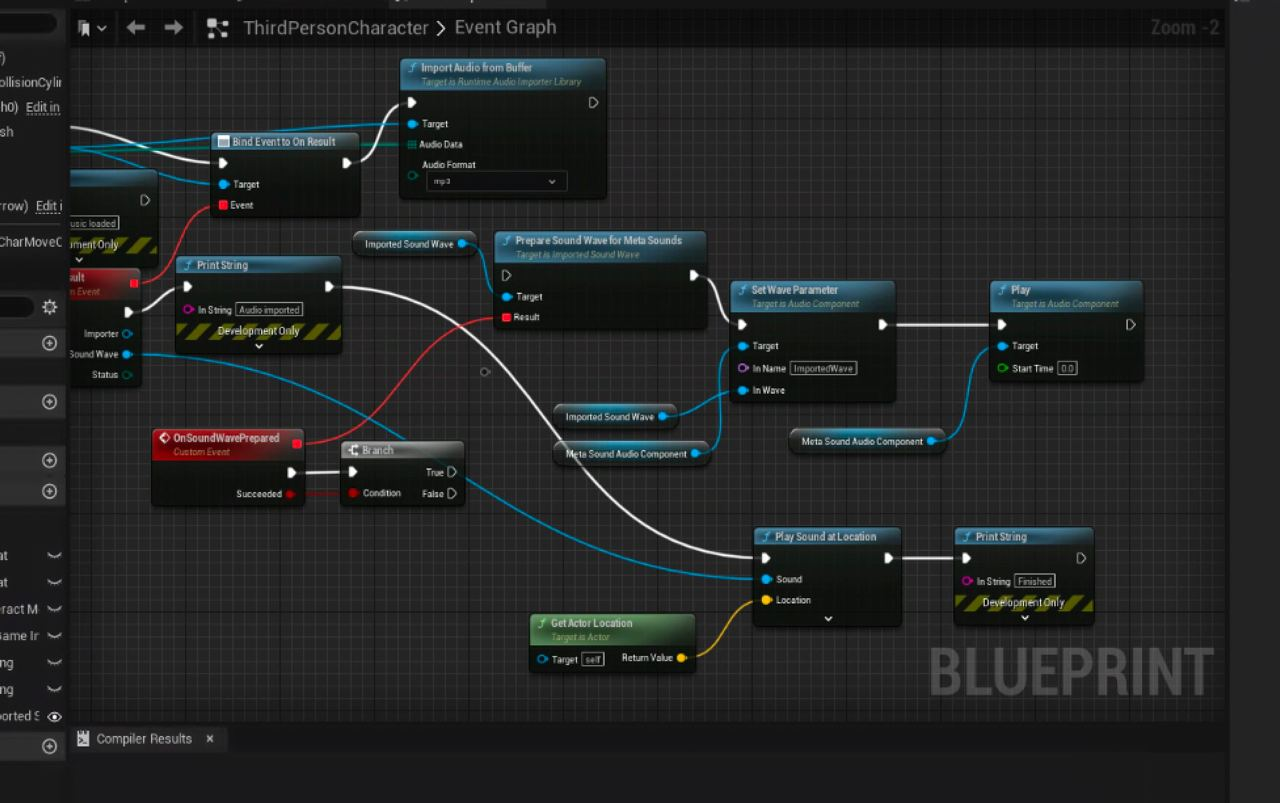
\includegraphics[scale=0.35]{gambar/blueprintfinal.jpg}

  % Ubah dengan keterangan gambar yang diinginkan
  \caption{Tampilan blueprint final}
  \label{fig:blueprintfinal}
\end{figure}
